\documentclass[9pt]{beamer}
\usepackage[UTF8]{ctex}
\usepackage{graphics}
\usepackage{amsmath}
\usepackage{xcolor} 
\usepackage{float}
\usefonttheme[onlymath]{serif}
\usepackage{subfig}
\usetheme{Warsaw}
%\usecolortheme{dolphin}
\setbeamercovered{transparent}
%%-------------------------------------------------
\title{工作汇报}
\author
{冯浩哲}

\date{2018 5.7}

\begin{document}
	\frame{\titlepage}

	%%-------------------------------------------------	
	
	\section*{展示大纲}
\begin{frame}[fragile]
	\frametitle{展示大纲}
	\begin{itemize}  
		
		\item 近期工作内容
		\vspace{0.3cm}
		\item 工作中所遇到的困难
		\vspace{0.3cm}
		\item 工作计划
		
	\end{itemize}
\end{frame}	


\section*{近期工作内容}
\begin{frame}[fragile]
	\frametitle{近期工作内容}
	我最近的工作主要是在做一个用于3D医学图像语义分割任务的无监督的Suggestive Annotation策略,其流程图如图所示:
	\begin{figure}[H]%
		\centering
		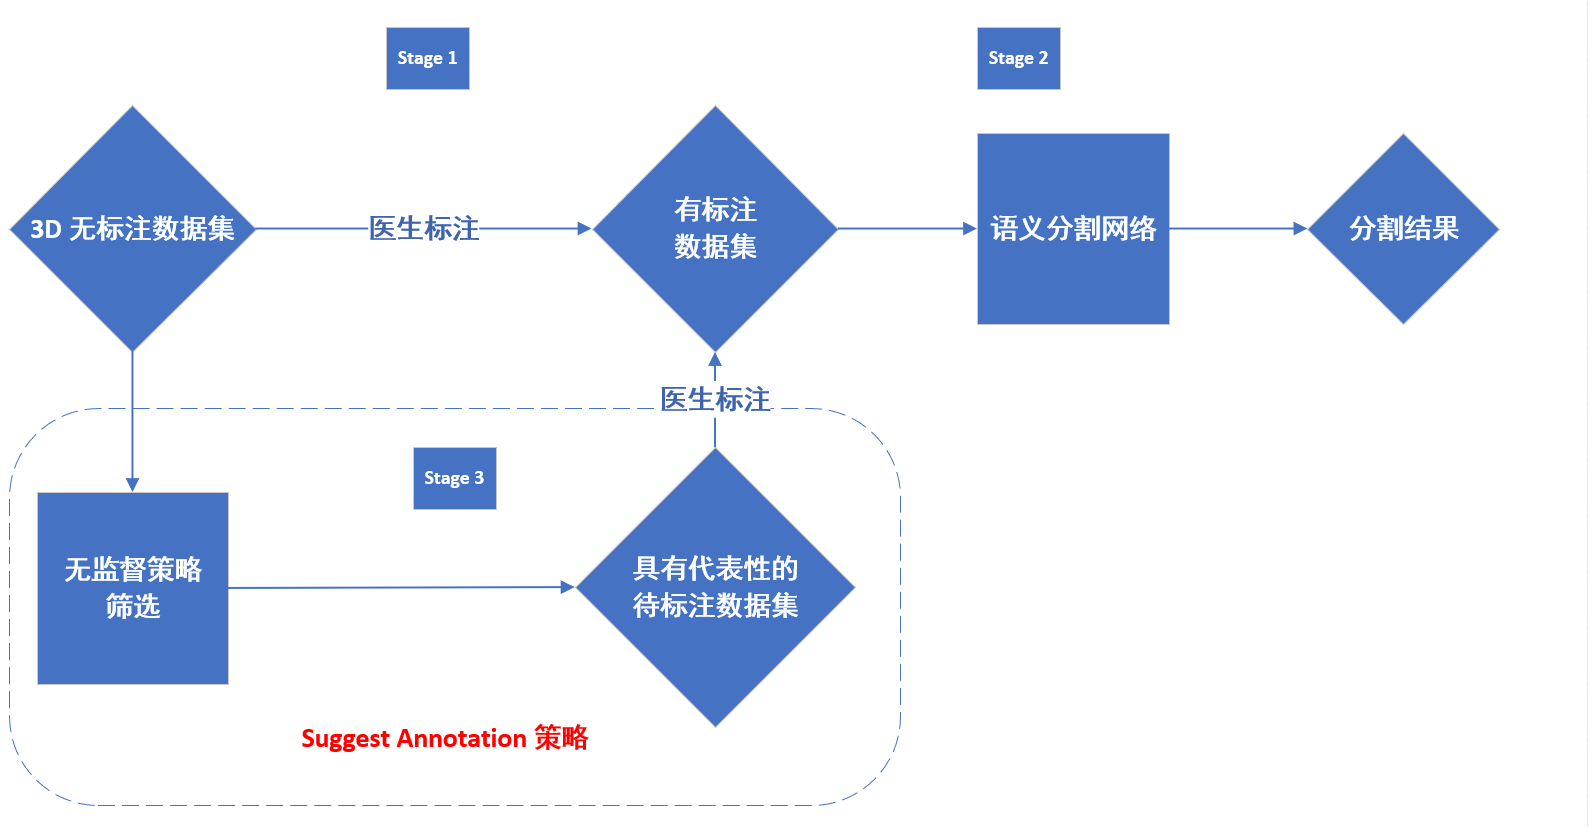
\includegraphics[width=10cm]{flowchart.png}%
	\end{figure}
	为了完成这个策略,我主要进行了3个阶段的工作:
\end{frame}

\begin{frame}[fragile]
	\frametitle{阶段性工作}
	\begin{itemize}
		\item[1] 从LIDC-IDRI数据集中构造了一个3D的肺结节数据集,每一个数据都有3D的语义分割标注


		\item[2] 设计了一个基于Densenet的语义分割网络来对3D肺结节数据集进行语义分割
	

		\item[3] 设计了一个无监督的Suggestive Annotation策略来筛选3D肺结节影像数据,从而减少语义分割任务所需的训练样本数目,减少标注负担
	\end{itemize}


\end{frame}


\begin{frame}[fragile]
	\frametitle{3D肺结节数据集介绍}
	我们从LIDC-IDRI数据集中构建了一个可以用于语义分割任务的3D肺结节数据集。这个肺结节数据集含有1148个肺结节,其中每一个数据都是$64*64*64$的cube,每一个体素的尺寸都是$1mm*1mm*1mm$,肺结节在cube的中心位置,如下图所示:
		\begin{figure}[H]%
			\centering
			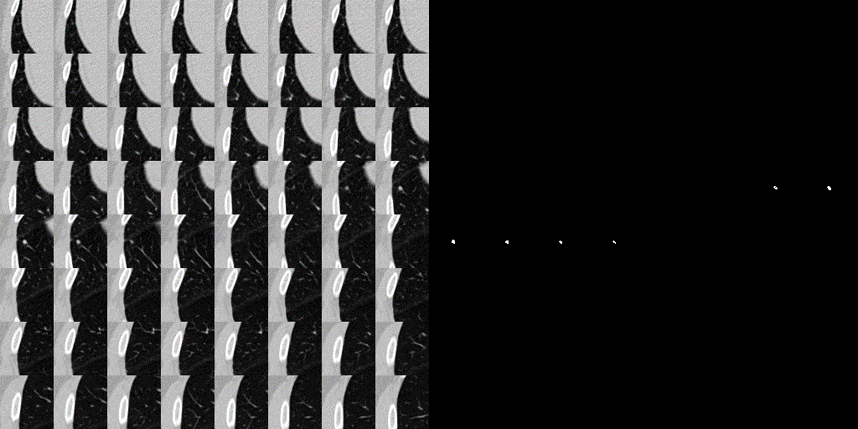
\includegraphics[width=8cm]{dataset.png}%
		\end{figure}
	该图把$64*64*64$的cube给展平为$8*8$的2D图像,每一块是一个slice。
\end{frame}

\begin{frame}[fragile]
	\frametitle{语义分割网络介绍}
	我们利用Densenet结构构建了一个用于3D肺结节语义分割的神经网络,如图所示:
		\begin{figure}[H]%
			\centering
			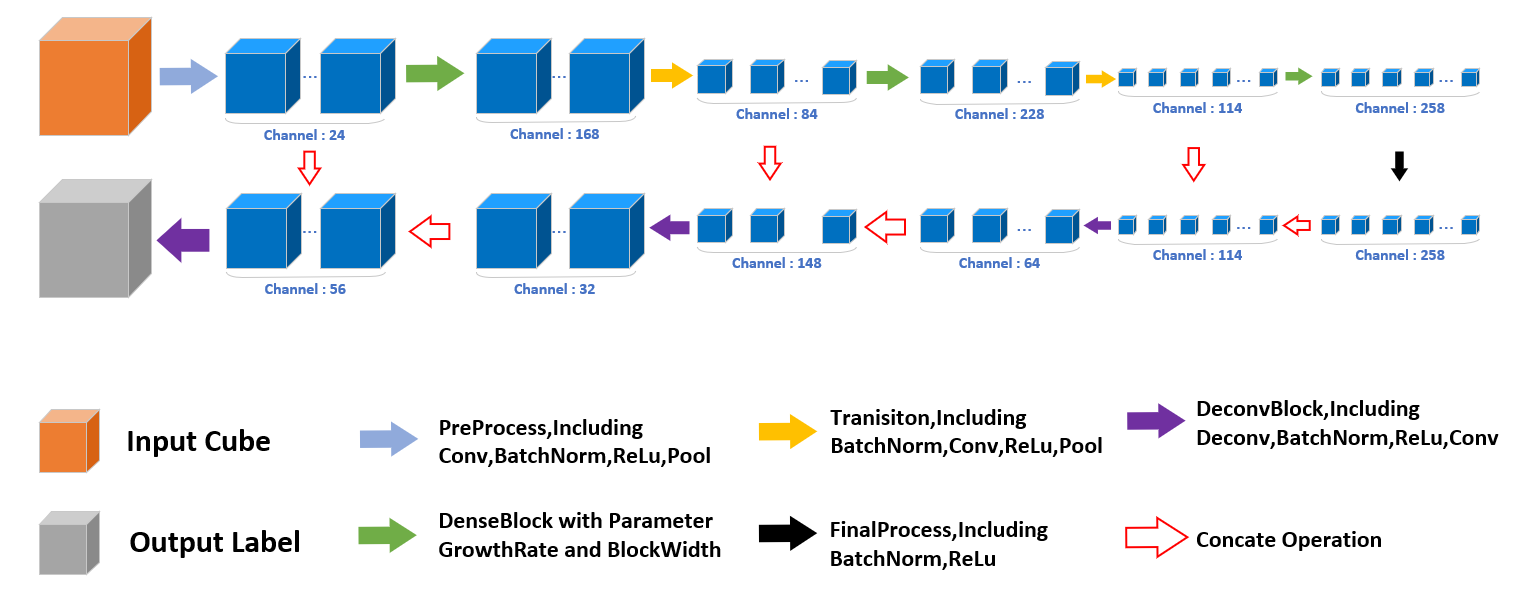
\includegraphics[width=8cm]{DenseSegnet.png}%
		\end{figure}
	它的输入是64*64*64的3D肺结节cube,输出的是一个肺结节的语义分割预测。我们将这个网络与现在在3D语义分割上做得最好的3D U-Net对比,
	这个网络只用了3D U-Net网络$\frac{1}{3}$的内存空间以及$\frac{1}{4}$的训练时间就可以收敛,而且能达到3D U-Net一样的结果。
	在我们的肺结节数据集上3D U-Net的结果是$Dice=0.763,VoE=0.37$,我们所构建的网络可以达到的结果是$Dice=0.757,VoE=0.373$。

\end{frame}

\begin{frame}[fragile]
	\frametitle{无监督Suggestive Annotation策略介绍}
	我们所提出的无监督Suggestive Annotation策略流程图如图所示:
	\begin{figure}[H]%
		\centering
		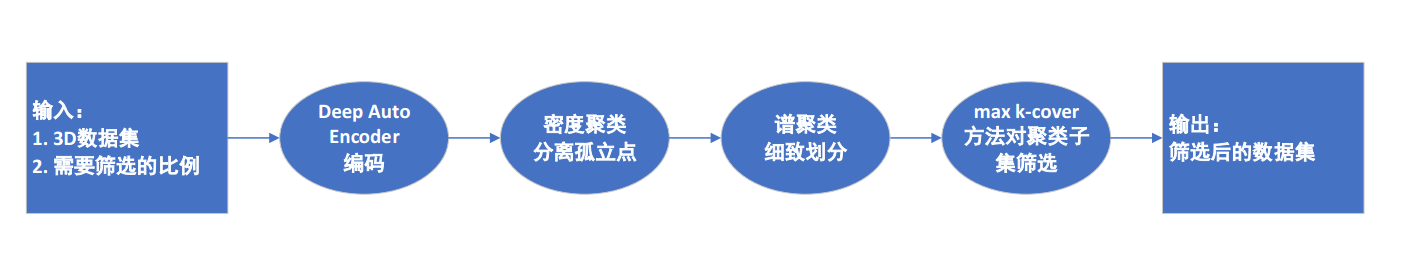
\includegraphics[width=12cm]{suggest_flow_chart.png}%
	\end{figure}
	我们将在下文以我们的3D肺结节数据集处理过程为例,简要概括这几个步骤。
	
\end{frame}

\begin{frame}[fragile]
	\frametitle{Deep Auto Encoder编码器}
	我们采用自动编码器进行特征提取。我们在3D肺结节数据集中用Deep Auto Encoder编码器将输入的每个$64*64*64$的cube映射到一个100维的向量,这是为了
	方便我们聚类。这个编码器的结构如图所示:
	\begin{figure}[H]%
		\centering
		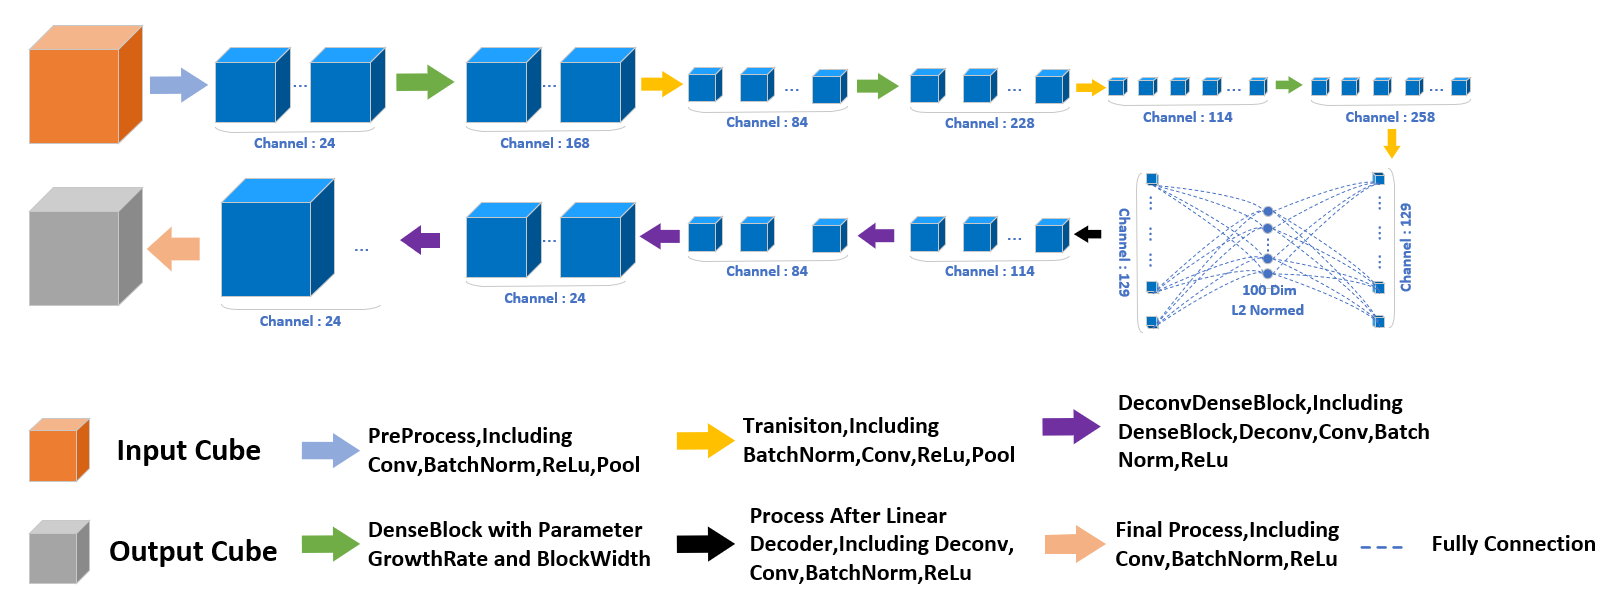
\includegraphics[width=12cm]{DenseEncoder.png}%
	\end{figure}
	它可以采用无监督的方式进行训练,损失函数是$loss=||X-Encoder(X)||_p$。
	
\end{frame}



\begin{frame}[fragile]
	\frametitle{密度聚类与谱聚类}
	获得肺结节的3D数据集所对应的1148个编码向量后,我们对这些编码向量进行聚类以代替直接对原数据集进行聚类。
	\begin{itemize}
		\item 用密度聚类进行预筛选
		
		以我们的肺结节3D数据集为例,我们希望从原来的1148个数据集中筛选出400个肺结节数据用于训练,那么我们采用密度聚类进行预筛选
		后将1148个数据集划分为n类+孤立点。我们的策略是选取所有的孤立点,然后从剩下的n类集合中使用谱聚类和max k-cover算法挑选具有代表性的数据。

		
	\end{itemize}

	
\end{frame}

\begin{frame}[fragile]
	\frametitle{密度聚类与谱聚类}
	获得肺结节的3D数据集所对应的1148个编码向量后,我们对这些编码向量进行聚类以代替直接对原数据集进行聚类。
	\begin{itemize}
		\item 用谱聚类进行进一步筛选

		我们采用谱聚类的方法对密度聚类的结果进行进一步筛选。以我们的肺结节3D数据集为例,我们需要对密度聚类所得到的n类集合进行等比例筛选,因此我们采用谱聚类对上述的数据集进行进一步划分,直到划分的每一个子集的数据集点的数目小于40。
		
	\end{itemize}

	
\end{frame}

\begin{frame}[fragile]
	\frametitle{max k-cover方法}
	在密度聚类和谱聚类的基础上,我们用Danny Chen教授所提出的max k-cover方法来进行具体的数据选取,如在我们的肺结节的3D数据集上,在经过密度聚类与谱聚类之后
	我们就需要面对如从含有40个数据的数据集中选4个数据出来的问题,在这个问题上max k-cover方法是一个好的策略。
\end{frame}


\section*{工作中遇到的困难}

\begin{frame}[fragile]
	\frametitle{工作中遇到的困难}
	我们在工作中主要遇到了2个困难:
	\begin{itemize}
	\item[1] LIDC 数据集没有提供测试集与验证集

	因为LIDC数据集并没有提供训练集,验证集,测试集的划分,如果我们需要得到一个实验结果,我们需要用5折交叉检验法,这个方法非常消耗时间。我们现在采用的方法是先用我们的完全无监督Suggest Annotation策略选取一些数据,然后把剩下的数据集作为测试集。
	我们也预计准备使用一些其它的公开数据集来测试我们的策略。
	\end{itemize}
\end{frame}

\begin{frame}[fragile]
	\frametitle{工作中遇到的困难}
	我们在工作中主要遇到了3个困难:
	\begin{itemize}
	\item[2] 对于自动编码器所得到的特征与分割结果好坏仍然无法建立显著性联系
	
	我们策略的基本假设是基于自动编码器所将原图(64*64*64)所映射到1个100维的向量能够描述原图的特征,即如果两个图像的编码向量彼此非常相似,那么两个图像的原图则具有非常相似的特征,从而我们能断言这两个图像只用标注一个就够了。我们经过实验发现,在测试集中分割得好的图像所对应的编码向量离训练集编码向量的平均距离一般会小于分割得不好的图像的平均距离,但是也有一些图像离训练集编码向量的平均距离很小,但是它们被分割得同样很糟糕。也就是两个图像的编码向量彼此相似并不代表着两个图像的分割结果也相似。
	\end{itemize}
\end{frame}



\begin{frame}[fragile]
	\frametitle{Danny Chen教授给出的建议}
	同时,Danny Chen教授也给我们的策略提出了4条问题与建议:
	\begin{itemize}
	\item[1] 我们所采用的聚类方法是否允许不同聚类之间的Overlapping
	\item[2] 对于那些只有几个数据的小类,比如孤立点问题,我们的聚类方法如何实现类别均衡的。
	\item[3] 对于从聚类结果中的数据选取,比如从600个数据集中选取60个数据集,这个选取的策略可以用最小支配集的方案来选取。
	\item[4] 尝试在选取原数据集60\%,50\%,40\%,...10\%的条件下对每一个百分比的最后结果画图,看看在选取不同百分比数据的时候我们的策略的表现。
	\end{itemize}
\end{frame}
\section*{工作计划}
\begin{frame}[fragile]
	\frametitle{工作计划}
	\begin{itemize}
		

	\item 短期工作目标

	完成毕业论文,预计5.15号之前完成

	\item 中期工作目标

	对Danny Chen教授所提出的建议进行尝试与实施。现在我们已经基于第一,三条建议对算法进行了改进,但是对第二个和第四个建议,即实现类别均衡问题以及在不同的百分比下绘图我们还会进行尝试。
	
	我们希望能对原算法进行改进,我们希望达到我们的策略比随机选的结果Dice要高出0.02以上,且测试结果Dice高于0.755。

	\item 长期工作目标

	将聚类算法用于Danny 提出的其它重要课题上,重新审视对抗策略。

	\item 投稿目标

	暂时目标定为11月的CVPR会议,但是我们不太确定自己这些基于医学影像的结果能不能投CVPR。
	\end{itemize}




\end{frame}
\end{document}